\documentclass[9pt]{beamer}

\usepackage{amsmath}
\usepackage{amsfonts}
\usepackage{listings}

\usepackage{graphicx}
\usepackage{ifpdf}
\ifpdf
  \DeclareGraphicsExtensions{.pdf,.png,.jpg}
\else
  \DeclareGraphicsExtensions{.eps}
\fi

\setbeamersize{text margin left=5mm,text margin right=5mm}
\setlength{\leftmargini}{3mm}
\setlength{\leftmarginii}{3mm}

% Temporarily change margin. https://tex.stackexchange.com/a/600
\def\changemargin#1#2{\list{}{\rightmargin#2\leftmargin#1}\item[]}
\let\endchangemargin=\endlist

\newcommand{\vect}[1]{\mathbf{#1}}
\newcommand{\pder}[2][]{\frac{\partial#1}{\partial#2}}
\newcommand\RR{\mathbb R}


\begin{document}

\begin{frame}
  \begin{center}
   Agenda
 \end{center}
 \begin{itemize}
 \item General pnlss settings
 \item Selecting multisine amplitude, ex: benchmark 4
 \item Validate PNLSS model using NFRC obtained by NLvib
 \item Use multiple amplitude data for estimation
 \item Can we trust NFRC obtained from discrete state space model?
 \end{itemize}
\end{frame}


\begin{frame}[fragile]{general PNLSS settings around 1 mode}
\begin{lstlisting}[language=matlab]
    % benchmark 1-3
    n = 2;
    whichtermsx = 'statesonly';
    whichtermsy = 'empty';
    nx = [3]    % benchmark 1/2
    nx = [2,3]  % benchmark 3
    % Benchmark 4
    n = 3;
    whichtermsx = 'full';
    whichtermsy = 'full';
    nx = [2,3];
    ny = [2,3];
    % benchmark 5
    n = 2;
    whichtermsx = 'full';
    whichtermsy = 'empty';
    nx = [2,3];
\end{lstlisting}

%   Nonlinear monomials
%   \begin{changemargin}{1cm}{0cm}
%   \begin{itemize}
%   \item[nx = [2,3]]: $x_1^2,x_1x_2,x_2^2$, $x_1^3,x_1^2x_2,x_1x_2^2,x_2^3$ $\rightarrow$ 23 parameters to estimate
%   \item[nx = [3]]: $x_1^3,x_1^2x_2,x_1x_2^2,x_2^3$ $\rightarrow$ 17 parameters
%   \end{itemize}
% \end{changemargin}
\end{frame}


\begin{frame}{Selecting MS amplitude - benchmark 4 example}
  \begin{itemize}
  \item Simulate with different amplitudes
  \item Inspect FRF and select amplitudes corresponding to fully stuck or fully sliding
  \item The expected frequencies are found from linear modal analysis of the
    two extremes.
  \end{itemize}

  \begin{center}
    Left: fully stuck; right: fully sliding\\
    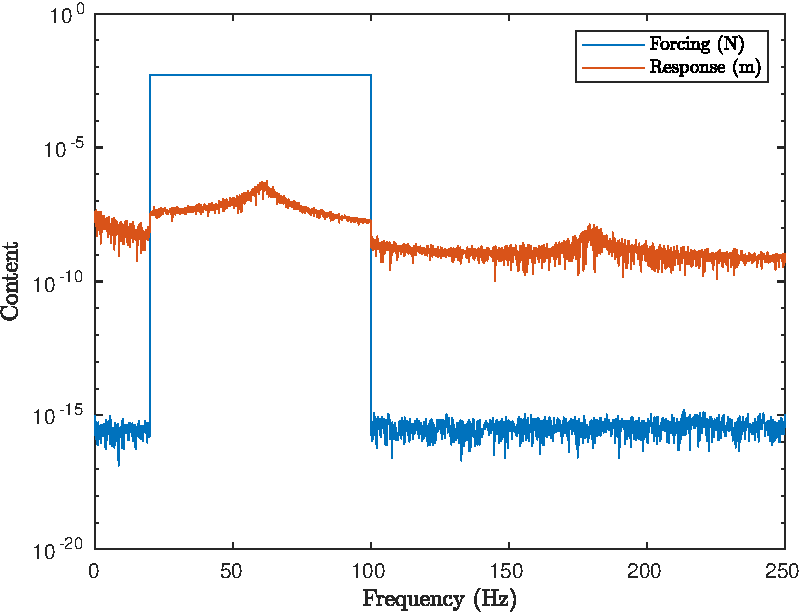
\includegraphics[width=0.45\textwidth]{fig/b4_famp01_ts}
    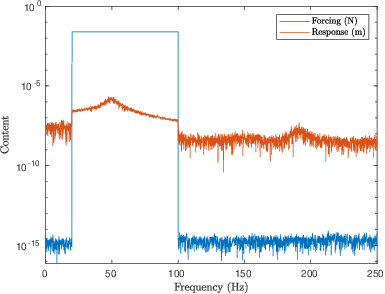
\includegraphics[width=0.45\textwidth]{fig/b4_famp05_ts}
  \end{center}
\end{frame}


\begin{frame}{Comparing NFRC: NLvib vs PNLSS}
  PNLSS estimated at A = 0.1 (low amplitude)
  \begin{itemize}
  \item Match well for lower amplitude (but damping overestimated)
  \item For increasing amplitude, the model 'blow up'
  \item As expected. Model is only valid within the range it was estimated
  \end{itemize}
  \begin{center}
    full line: PNLSS; thin line: NLvib\\
    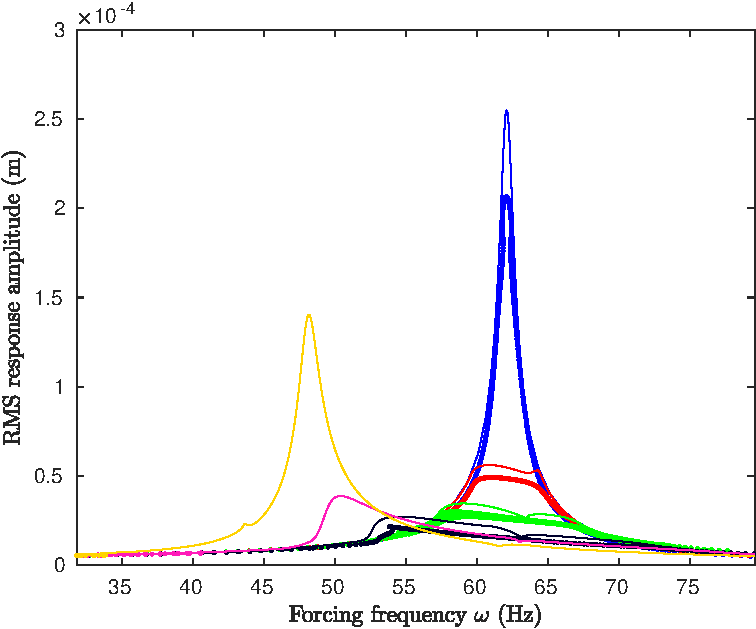
\includegraphics[width=0.45\textwidth]{fig/b4_pnlssfrf_A01_Amp}
    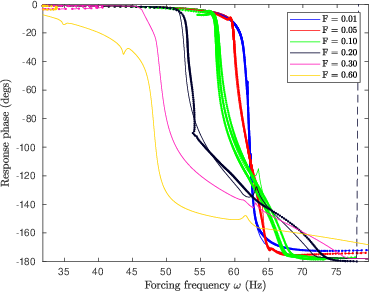
\includegraphics[width=0.45\textwidth]{fig/b4_pnlssfrf_A01_Phase}
  \end{center}
\end{frame}


\begin{frame}{Comparing NFRC: NLvib vs PNLSS}
  PNLSS estimated at A = 0.5 (high amplitude)
  \begin{itemize}
  \item Match for forcing resulting in microslip, $F=0.2$ \& $F=0.3$
  \item For all other forcing levels, the behavior is unpredictable
  \end{itemize}
  \begin{center}
    full line: PNLSS; thin line: NLvib\\
    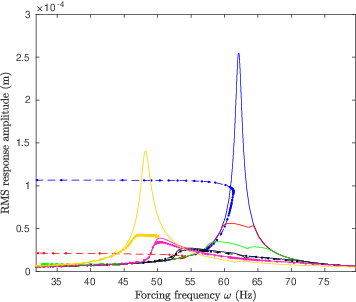
\includegraphics[width=0.45\textwidth]{fig/b4_pnlssfrf_A05_Amp}
    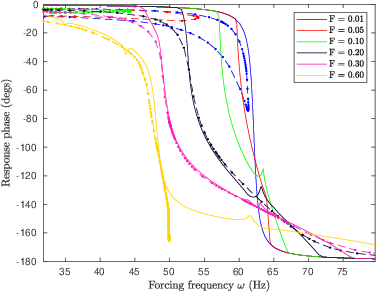
\includegraphics[width=0.45\textwidth]{fig/b4_pnlssfrf_A05_Phase}
  \end{center}
\end{frame}


\begin{frame}{Estimate model from combined data}
  Combine low and high amplitude data for estimating
  \begin{itemize}
  \item Linear model gives a poor fit.
  \item Keep 3 state model. Misfit to BLA is due to nonlinearity.
  \item Nonlinear model seems to perform well on this particular data
  \end{itemize}
  \begin{center}
    left: Subspace; right: Estimation, time domain\\
    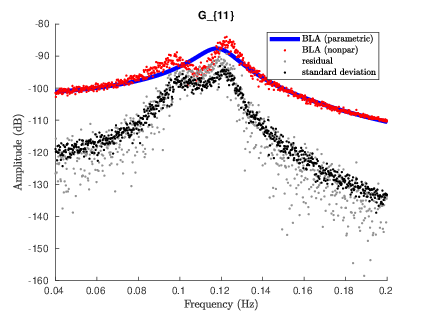
\includegraphics[width=0.45\textwidth]{fig/PNLSS_comb_BLA_parnonpar}
    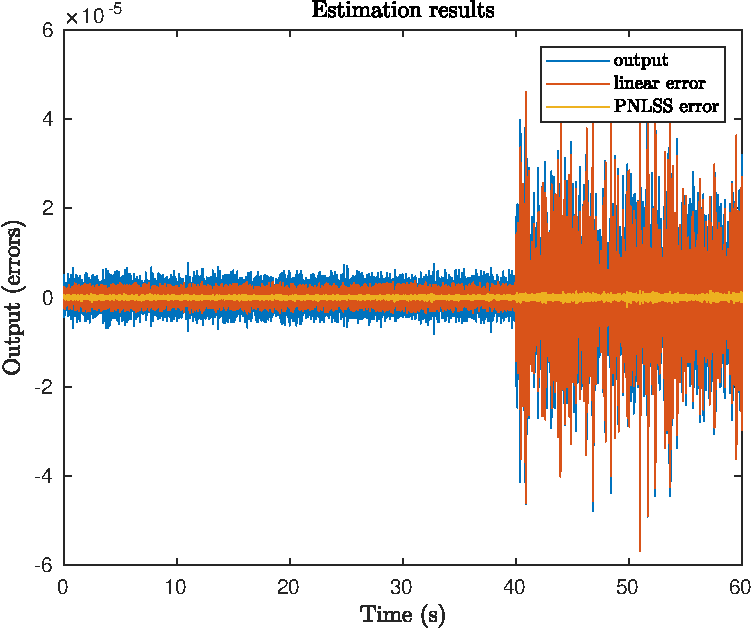
\includegraphics[width=0.45\textwidth]{fig/PNLSS_comb_TDOMRES}
  \end{center}
\end{frame}


\begin{frame}{Comparing NFRC: NLvib vs PNLSS}
  Combine low and high amplitude data for estimating
  \begin{itemize}
  \item Poor performance for all excitation levels
  \end{itemize}
  \begin{center}
    full line: PNLSS; thin line: NLvib\\
    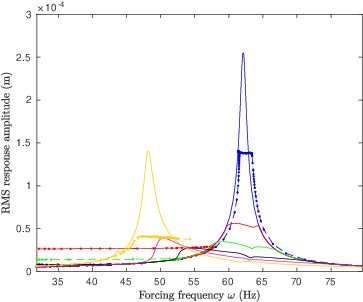
\includegraphics[width=0.45\textwidth]{fig/pnlssfrf_Acomb_Amp}
    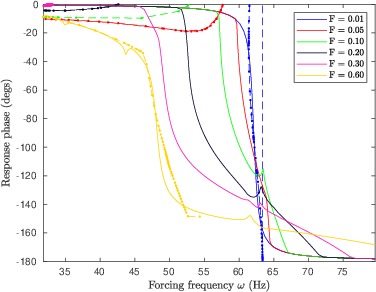
\includegraphics[width=0.45\textwidth]{fig/pnlssfrf_Acomb_Phase}
  \end{center}
\end{frame}


\begin{frame}{Alternative data covering all amplitudes}
  Let amplitude vary linearly from low to high - Arrowhead.
  \begin{itemize}
  \item But frequency content destroyed when signal is not periodic
  \item Thus (we assume) not suitable for training. Maybe for model selecting.
  \end{itemize}
  \begin{center}
    Left: repeated arrow-head; right: zoom at $t=T$; bottom: frequency content\\
    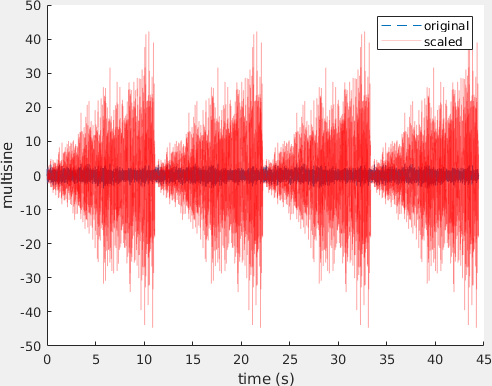
\includegraphics[width=0.4\textwidth]{fig/arrow_full}
    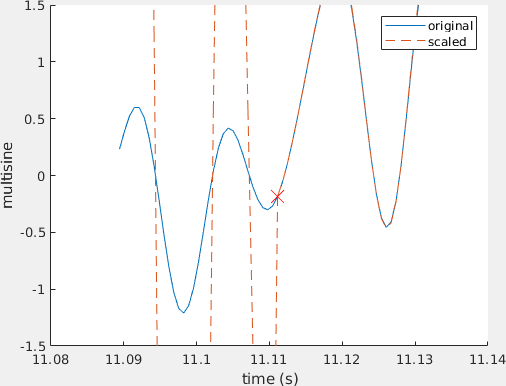
\includegraphics[width=0.4\textwidth]{fig/arrow_zoom}
    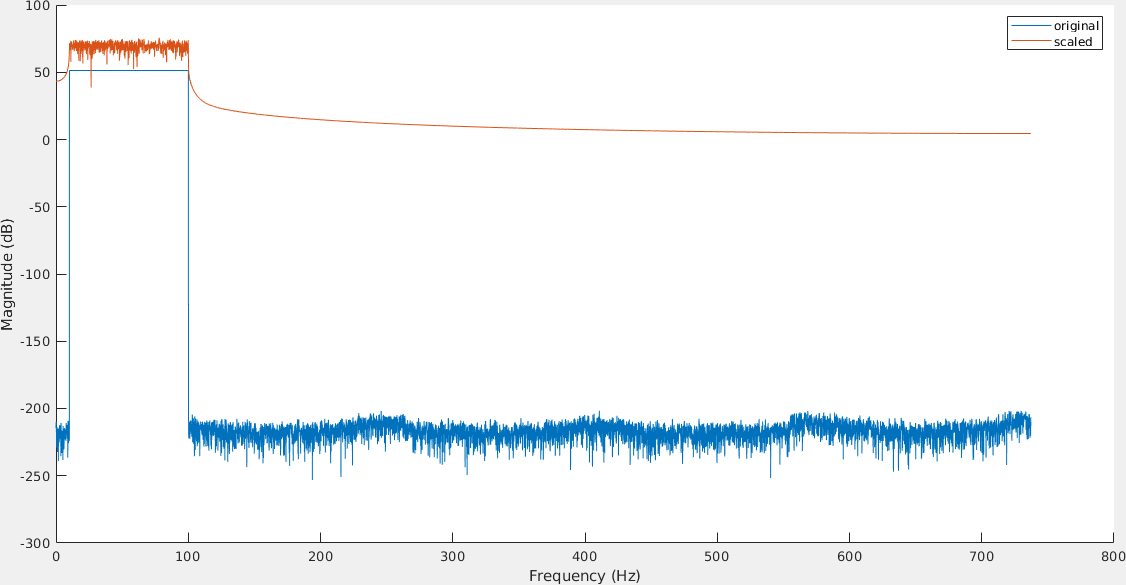
\includegraphics[width=0.55\textwidth]{fig/arrow_freq}
  \end{center}
\end{frame}


\begin{frame}{Can we trust NFRC and phase from discrete time PNLSS?}
  We evaluate PNLSS performance based on NFRC and phase plot. But can we trust
  these plots?\\
  Next slides show NFRC and phases computed from discrete time state space model
  for the duffing oscillator. The discretisation is done at different $fs$\\
  The same behavior is seen for a linear ss model, where the conversion at a
  given $fs$ is exact; ie. it can not only be attributed to the euler
  discretization of the nonlinearity.\\
  Thin line is 'analytical model', dotted is discrete time state space.
  \begin{itemize}
  \item poor agreement
  \end{itemize}
  \begin{center}
    $fs=2^{12}=4096 Hz$\\
    Left: NFRC; Right: Phase\\
    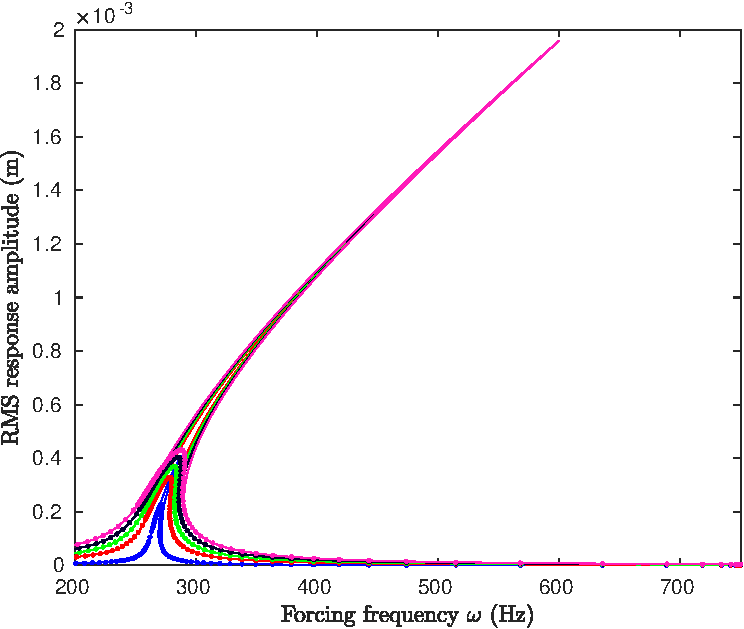
\includegraphics[width=0.45\textwidth]{fig/nfrc/dssex_frf_Amp_fs4096}
    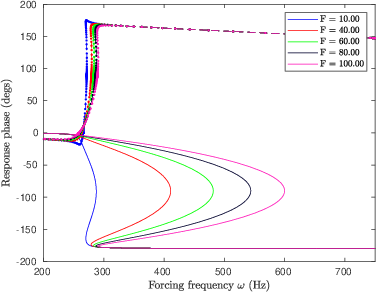
\includegraphics[width=0.45\textwidth]{fig/nfrc/dssex_frf_Phase_fs4096}
  \end{center}
\end{frame}


\begin{frame}{$fs=2^{16}=65536 Hz$}
  \begin{itemize}
  \item poor agreement
  \end{itemize}
  \begin{center}
    Left: NFRC; Right: Phase\\
    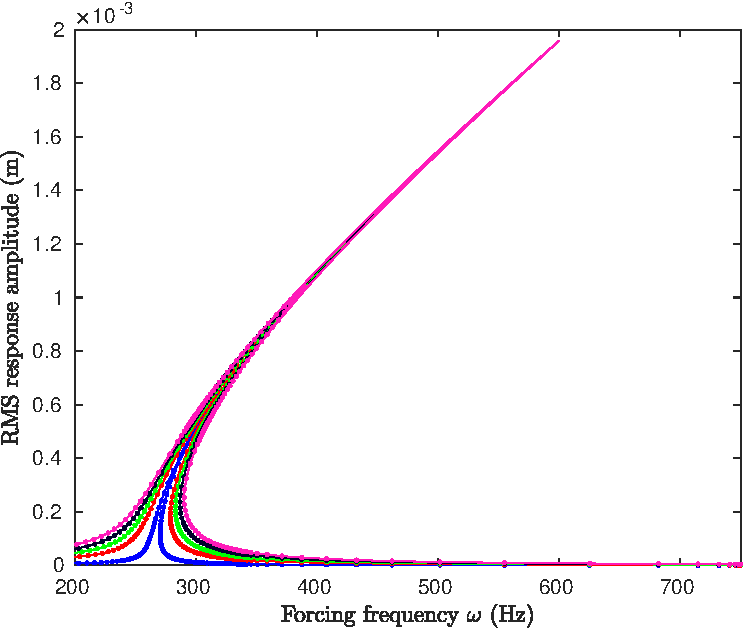
\includegraphics[width=0.45\textwidth]{fig/nfrc/dssex_frf_Amp_fs65536}
    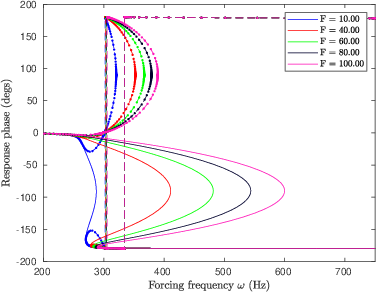
\includegraphics[width=0.45\textwidth]{fig/nfrc/dssex_frf_Phase_fs65536}
  \end{center}
\end{frame}



\begin{frame}{$fs=2^{20}=1048576 Hz$}
  \begin{itemize}
  \item Match for lowest force
  \end{itemize}
  \begin{center}
    Left: NFRC; Right: Phase\\
    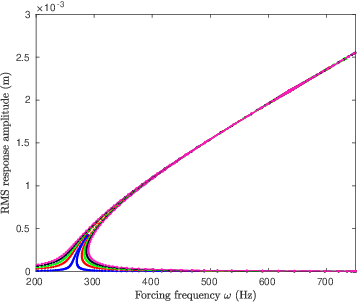
\includegraphics[width=0.45\textwidth]{fig/nfrc/dssex_frf_Amp_fs1048576}
    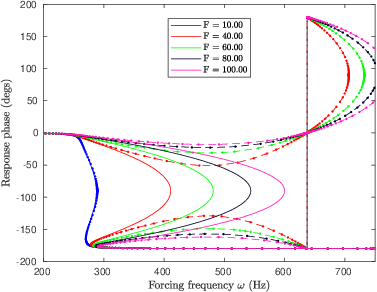
\includegraphics[width=0.45\textwidth]{fig/nfrc/dssex_frf_Phase_fs1048576}
  \end{center}
\end{frame}


\begin{frame}{$fs=2^{20}=1048576 Hz$}
  \begin{itemize}
  \item Match for lowest force
  \end{itemize}
  \begin{center}
    Left: NFRC; Right: Phase\\
    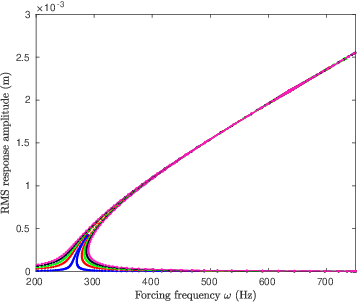
\includegraphics[width=0.45\textwidth]{fig/nfrc/dssex_frf_Amp_fs1048576}
    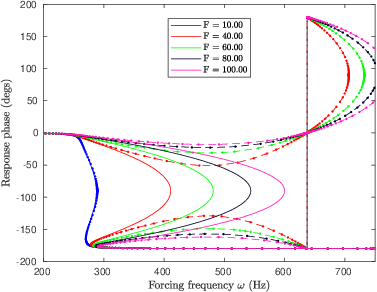
\includegraphics[width=0.45\textwidth]{fig/nfrc/dssex_frf_Phase_fs1048576}
  \end{center}
\end{frame}


\begin{frame}{$fs=2^{21}=2097152 Hz$}
  \begin{itemize}
  \item Starting to get better
  \end{itemize}
  \begin{center}
    Left: NFRC; Right: Phase\\
    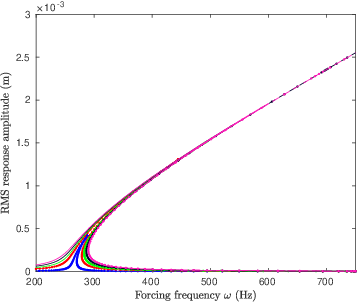
\includegraphics[width=0.45\textwidth]{fig/nfrc/dssex_frf_Amp_fs2097152}
    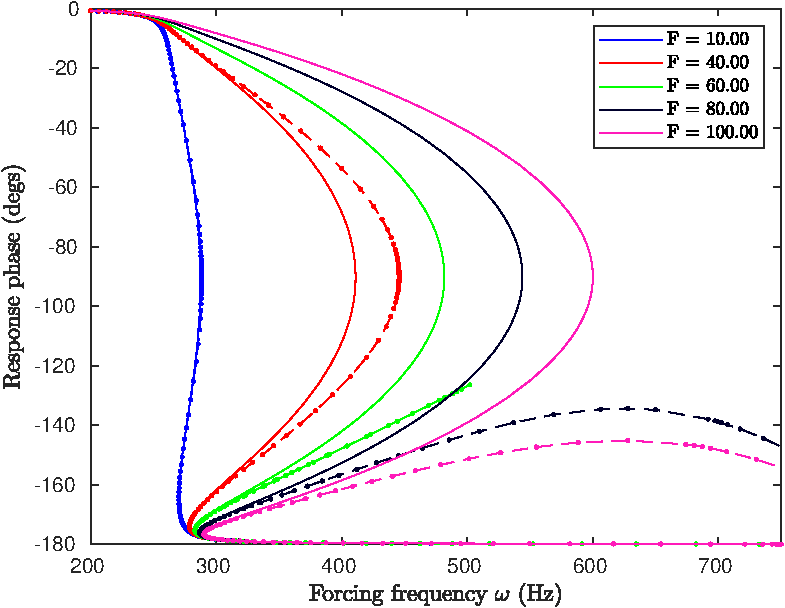
\includegraphics[width=0.45\textwidth]{fig/nfrc/dssex_frf_Phase_fs2097152}
  \end{center}
\end{frame}


\begin{frame}{$fs=2^{22}=4194304 Hz$}
 \begin{center}
    Left: NFRC; Right: Phase\\
    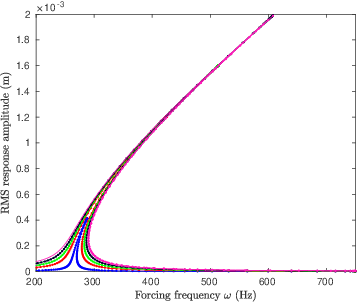
\includegraphics[width=0.45\textwidth]{fig/nfrc/dssex_frf_Amp_fs4194304}
    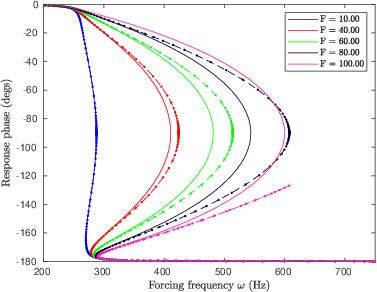
\includegraphics[width=0.45\textwidth]{fig/nfrc/dssex_frf_Phase_fs4194304}
  \end{center}
\end{frame}


\begin{frame}{$fs=2^{24}=16777216 Hz$}
 \begin{center}
    Left: NFRC; Right: Phase\\
    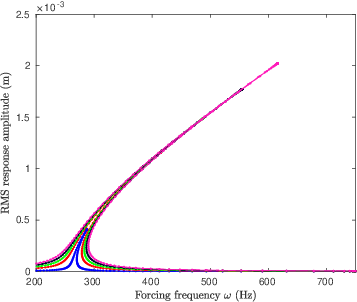
\includegraphics[width=0.45\textwidth]{fig/nfrc/dssex_frf_Amp_fs16777216}
    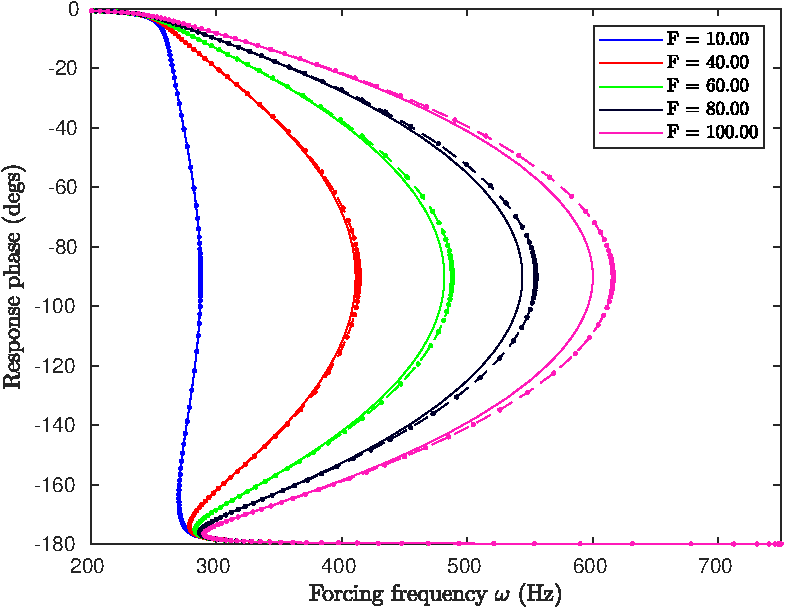
\includegraphics[width=0.45\textwidth]{fig/nfrc/dssex_frf_Phase_fs16777216}
  \end{center}
\end{frame}


\begin{frame}{$fs=2^{28}=268435456 Hz$}
  At a sampling frequency of 268 million Hz, there is good agreement.\\
  This raises the question: At which sampling frequency shall we identify the
  PNLSS model?
 \begin{center}
    Left: NFRC; Right: Phase\\
    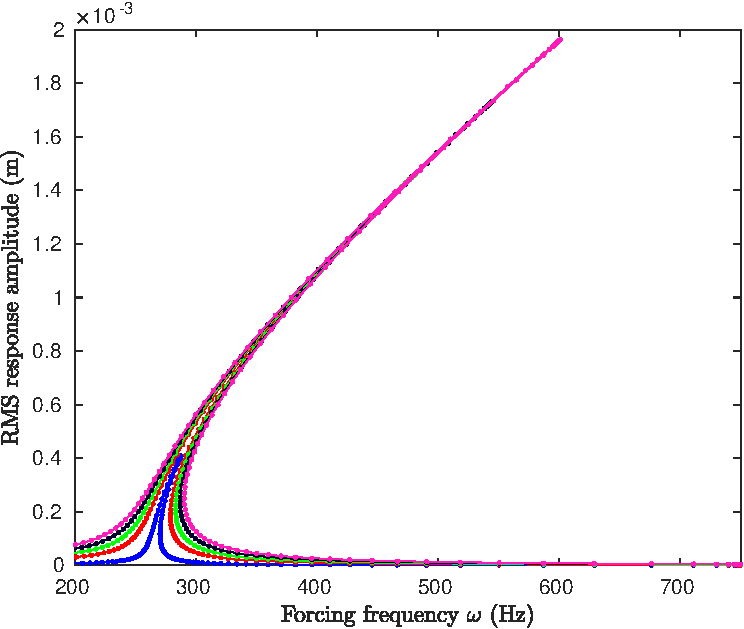
\includegraphics[width=0.45\textwidth]{fig/nfrc/dssex_frf_Amp_fs268435456}
    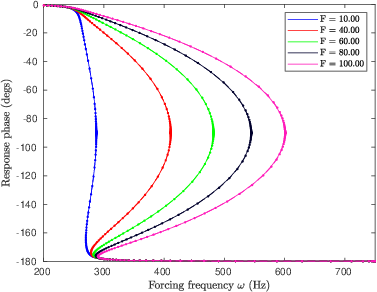
\includegraphics[width=0.45\textwidth]{fig/nfrc/dssex_frf_Phase_fs268435456}
  \end{center}
\end{frame}

\begin{frame}
  \frametitle{Linear System: Continuous vs Discretized}
  \framesubtitle{Continuous time HB vs Discrete time HB}
  \begin{itemize}
  \item Considering just the linear part of the above system, FRF
    studies were carried out for different $fs$
  \end{itemize}
  \begin{center}
    $fs = 2^{12} = 4096 Hz$\\
   Left: NFRC; Right: Phase\\
   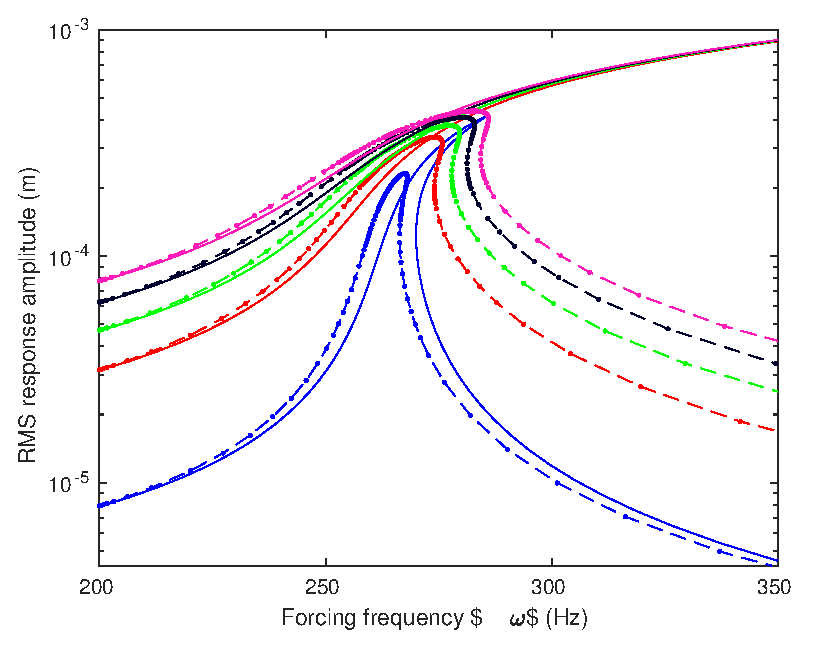
\includegraphics[width=0.45\textwidth]{../../benchmark0/fig/dssex_frf_Amp_fs4096}
   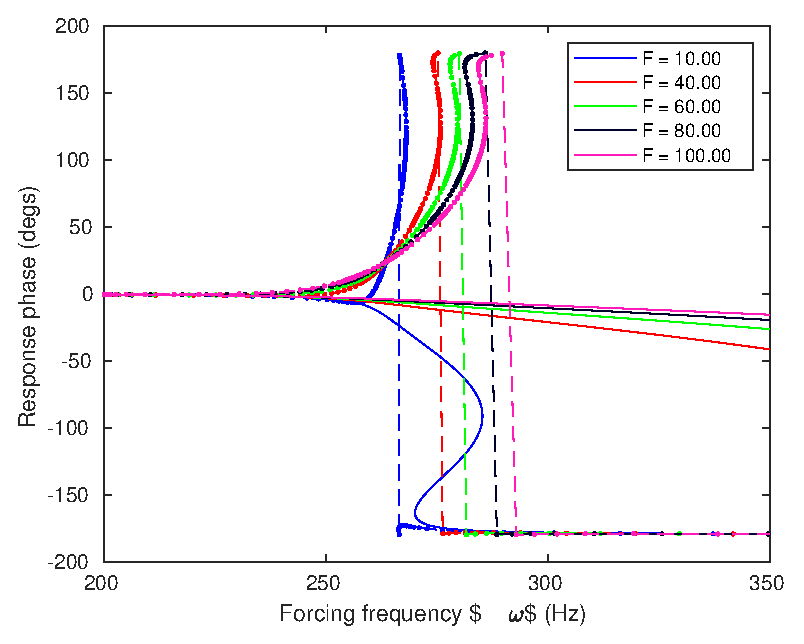
\includegraphics[width=0.45\textwidth]{../../benchmark0/fig/dssex_frf_Phase_fs4096}
  \end{center}  
\end{frame}

\begin{frame}
  \frametitle{Linear System: Continuous vs Discretized}
  \framesubtitle{Continuous time HB vs Discrete time HB}
  \begin{itemize}
  \item Considering just the linear part of the above system, FRF
    studies were carried out for different $fs$
  \end{itemize}
  \begin{center}
    $fs = 2^{18} = 262,144 Hz$\\
   Left: NFRC; Right: Phase\\
   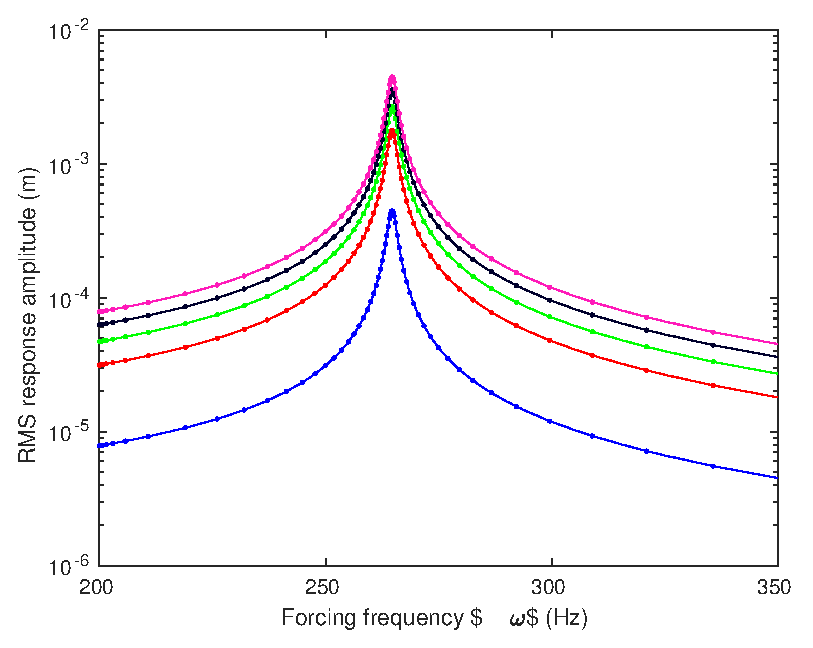
\includegraphics[width=0.45\textwidth]{../../benchmark0/fig/dssex_frf_Amp_fs262144}
   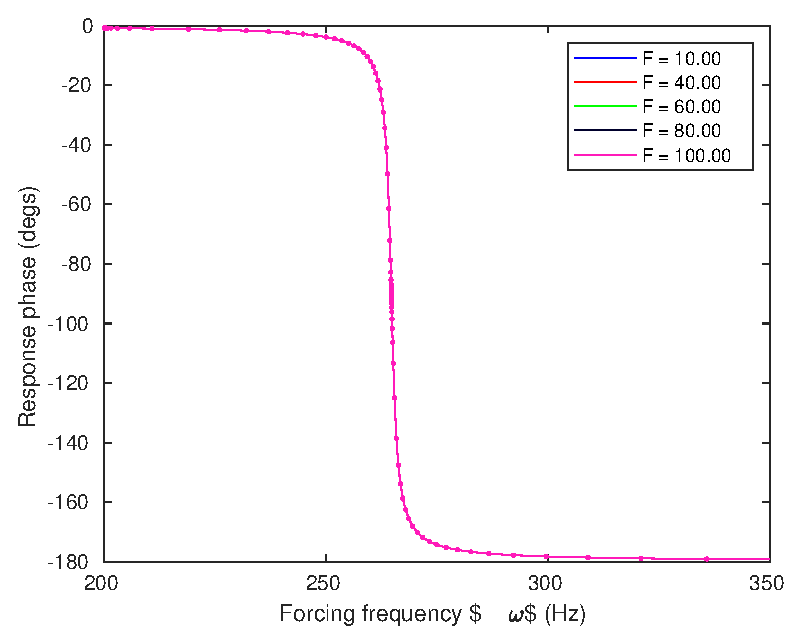
\includegraphics[width=0.45\textwidth]{../../benchmark0/fig/dssex_frf_Phase_fs262144}
  \end{center}  
\end{frame}

\begin{frame}
  \frametitle{Linear System: Continuous vs Discretized}
  \framesubtitle{Continuous time HB vs Discrete time MARCHING}
  \begin{itemize}
  \item Considering just the linear part of the above system, FRF
    studies were carried out for different $fs$
  \end{itemize}
  \begin{center}
    $fs = 2^{12} = 4096 Hz$\\
   Left: NFRC; Right: Phase\\
   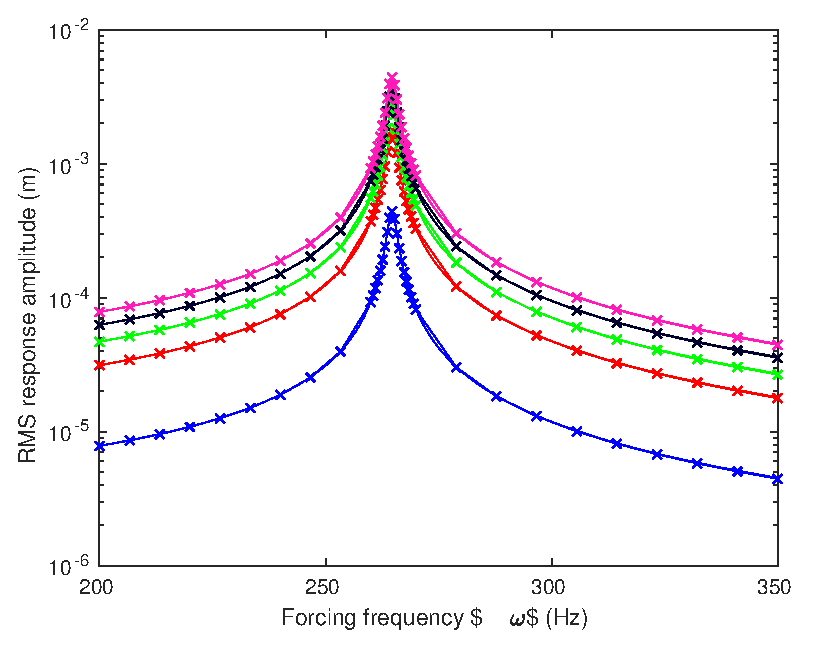
\includegraphics[width=0.45\textwidth]{../../benchmark0/fig/TMdssex_frf_Amp_fs4096}
   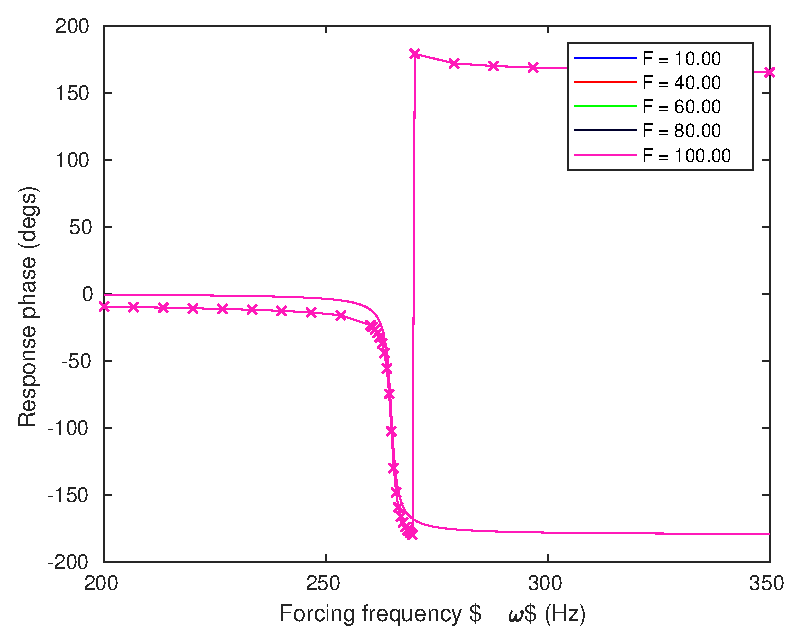
\includegraphics[width=0.45\textwidth]{../../benchmark0/fig/TMdssex_frf_Phase_fs4096}
  \end{center}  
\end{frame}

\begin{frame}
  \frametitle{Linear System: Continuous vs Discretized}
  \framesubtitle{Continuous time HB vs Discrete time MARCHING}
  \begin{itemize}
  \item Considering just the linear part of the above system, FRF
    studies were carried out for different $fs$
  \end{itemize}
  \begin{center}
    $fs = 2^{18} = 262,144 Hz$\\
   Left: NFRC; Right: Phase\\
   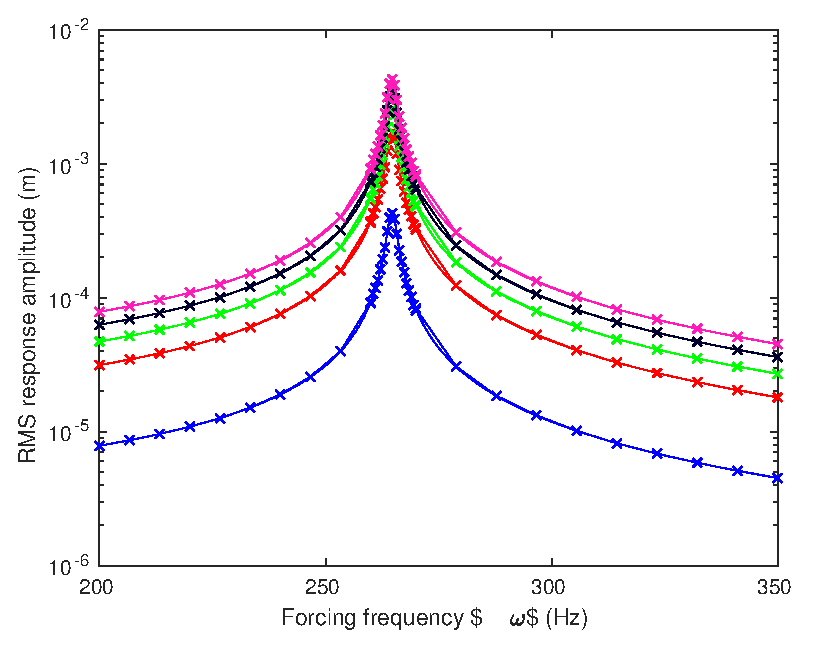
\includegraphics[width=0.45\textwidth]{../../benchmark0/fig/TMdssex_frf_Amp_fs262144}
   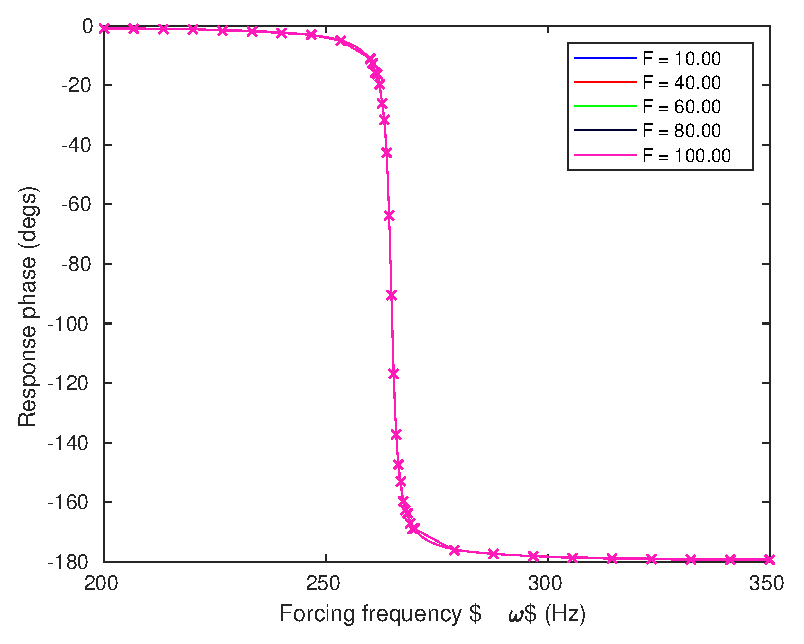
\includegraphics[width=0.45\textwidth]{../../benchmark0/fig/TMdssex_frf_Phase_fs262144}
  \end{center}  
\end{frame}

\begin{frame}
  \frametitle{Consistency of PNLSS}
  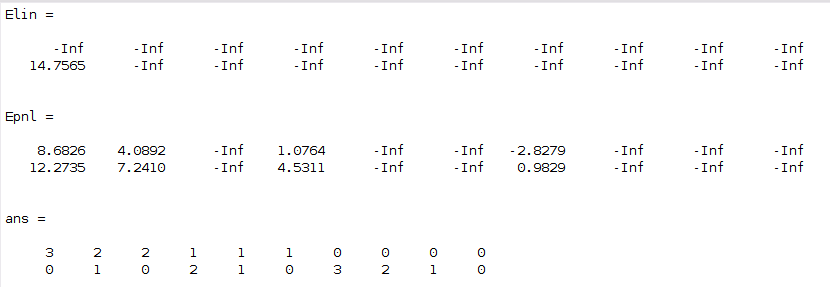
\includegraphics[width=0.8\textwidth]{./fig/consist}
\end{frame}

% \begin{frame}<1>[label=pnlss]
%   \begin{center}
%     \visible<1>{Steps taken so far with PNLSS modeling}
%   \end{center}
%   \alert<1>{Generate data} \newline
%   \alert<2>{Consistency} \newline
%   \alert<3>{Nonparametric analysis} \newline
%   \alert<4>{Parametric modeling}
% \end{frame}

% \begin{frame}[fragile]{general PNLSS settings around 1 mode}

% \begin{lstlisting}[language=matlab]
%     % benchmark 1-3
%     n = 2;
%     whichtermsx = 'statesonly';
%     whichtermsy = 'empty';
%     nx = [3]    % benchmark 1/2
%     nx = [2,3]  % benchmark 3
%     % Benchmark 4

% \end{lstlisting}
%   Nonlinear monomials
%   \begin{itemize}
%   \item[$nx = [2,3]$]: $x_1^2,x_1x_2,x_2^2$, $x_1^3,x_1^2x_2,x_1x_2^2,x_2^3$ $\rightarrow$ 23
%     parameters to estimate
%   \item[$nx = [3]$]: $x_1^3,x_1^2x_2,x_1x_2^2,x_2^3$ $\rightarrow$ 17 parameters
%   \end{itemize}


% \end{frame}

% \begin{frame}[fragile]{Noise}
%   \begin{itemize}
%   \item SNR?
%   \item Type/color?
%   \end{itemize}

%   \begin{lstlisting}
%     noise = 1e-3*std(y(:,end,end))*randn(size(y));
%     % Do some filtering
%     noise(1:end-1,:,:) = noise(1:end-1,:,:) + noise(2:end,:,:);
%   \end{lstlisting}
%   \begin{center}
%   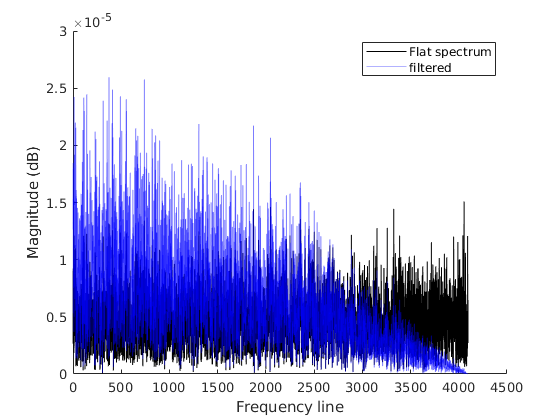
\includegraphics[width=0.55\textwidth]{fig/noise}
% \end{center}
% \end{frame}


% e_est_lin:	 1.860e-05	 e_est_nl:	 7.570e-08
% e_val_lin:	 1.639e-05	 e_val_nl:	 7.465e-08
% e_test_lin:	 1.530e-05	 e_test_nl:	 4.152e-06

% Nat freq 264.72, 264.72,  Hz.
% damping 0.003798

% 264.7179


% Identified Modal Parameters
% Nat freq 265.76, 265.76,  Hz.
% damping 0.0037382, 0.0037382,

\end{document}

%%% Local Variables:
%%% mode: latex
%%% coding: utf-8-unix
%%% TeX-engine: luatex
%%% magic-latex-enable-block-highlight: nil
%%% TeX-master: t
%%% End: